 Couchbase Server is designed to access real-time operational data. It is a NoSQL database that serves both as key-value and document-oriented database. As a key-value store, it is able to store any type of data including  strings, numbers and binary data and the data is treated as an opaque Binary Large Object(BLOB). When used as document store, data is stored in a valid JSON format. The data is stored in logical unit called buckets. These buckets are isolated to each other and have their own RAM quota and replica settings. Buckets can be compared with \texttt{database} of MongoDB or any other RDBMS. Couchbase recommends few number of buckets in a single cluster. 
 \todo{write about raplica settings and ram quota}
 
 \subsubsection{Data Model}%repeat check once
 
The data model of Couchbase is different than other NoSQL databases. The data is stored in the form of key/value pair inside a bucket. Individual documents are indentified by its key called Document ID. A bucket can contain any type of data but other than JSON type can be retrieved only by its key. Therefore, before fetching, it is important to check metadata \textit{type} that is stored with a single document. Each document is stored independently and there is no notion of grouping of documents like collections in MongoDB or tables in other RDBMS. An user-defined type attribute can be created to differentiate the various documents stored in the bucket and  create indexes on them.  For example, \textit{user} and \textit{post} are two collections of MongoDB. The documents of these two collections can be represented in Couchbase by adding a new field \textit{documentType}  in each document with value \textit{user} and \textit{post} respectively. 

\paragraph{RAM Quota}
It is necessary to define the amount of memory for Server and individual bucket in Couchbase before storing data. 
\begin{itemize}
\item {Server quota:}
          Server quota is allocated when Couchbase server is first installed. The amount of RAM allocation depends on per-node basis. The quota is identical to all the nodes. For instance, if there are 8 nodes with AND A 16GB Server quota, there is 144GB RAM available across the cluster. Further addition of 2 nodes to the cluster and the new nodes would need 16GB of free RAM, in total the RAM available in the cluster would be 160GB.   
\item{Bucket quota:}    
For data caching, certain amount of RAM should be allocated to an individual bucket. These bucket quotas are on per-node basis. For example, when a new bucket is created with a bucket quota of 1GB, in a 8 node cluster then in total there would be 8GB of bucket quota in the cluster. By adding 2 more nodes to the cluster would extend bucket quota to 10GB. 
\end{itemize}
           
\paragraph{Metadata}\label{cb-metadata}
%may be we can remove it.
For every value stored in a bucket, Couchbase generates following meta information that is associated with a document~\cite[p. 26]{cb/ostrovsky2014pro}. 
\begin{itemize}
	\item{Expiration time:}
		The Time to Live(TTL) also named as expiration time is the life time of a document. The default value of TTL is 0 that indicates document will never expire and also can be set as Unix epoch time after which document is removed.
	\item{Check-and-Set(CAS):}
		The CAS value is 64-bit integer that is updated by the server when associated item is modified. The document is updated only  if unique identifier matches the identifier of the document. CAS is used to manage concurrency when multiple client attempts to update the same document simultaneously. 
	\item{Flags:} 
Flags are SDK-specific parameter that are used to identify the format and the type of data objects being stored.
\item{Type:}
 \textit{type} is the type of a document either \textit{json} or Base64 encoded string.
 \item{Document Key:}
 Every value in Couchbase is saved with unique identifier called document key. Unlike MongoDB, in Couchbase the key should be manually generated. The key length should be with in 250 characters.
\end{itemize}	

%In case of XMark data each \texttt{id} attributes of  \texttt{item}, \texttt{person}, \texttt{open\_auction}, \texttt{category} represent as key. In case of  \texttt{closed\_auction} and  \texttt{edge} key can be manually generated. 
\begin{figure}[h]
	\centering
	\subfloat[Views in Document Design]{
		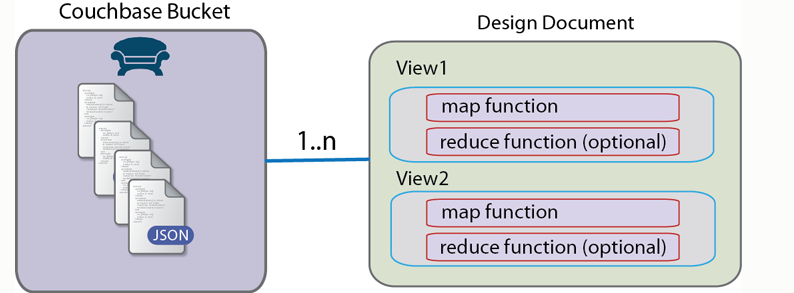
\includegraphics[width=0.4\textwidth]{img/cb/Small_view_elements}
		\label{fig:cb-views-design}
	}
	\centering
	\subfloat[View's Workflow]{
		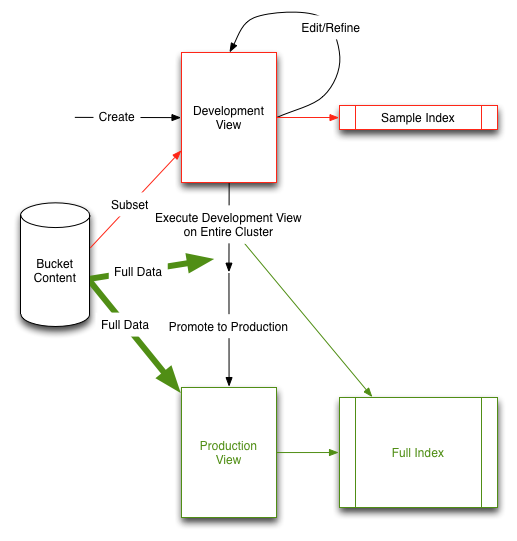
\includegraphics[width=0.4\textwidth]{img/cb/view-types-workflow}
		\label{fig:cb-views-workflow}
	}
	\caption{Couchbase Server's Document Design ~\citep{couchbasedocs}}
	\label{fig:cb-views-document-design}	
\end{figure}

\paragraph{Bucket and vBucket}
 Data bucket used by the Couchbase is a logical container of information that provides a logical grouping of physical resources within a cluster~\citep{lichtenberg2013nosql}. Documents in Couchbase do not have fixed structure. Each bucket is split into 1024 logical partitions called vBuckets. A vBucket is treated as a owner of subset of keys as shown in Figure~\ref{fig:cb-vbucket}.  
%%why we need vbucket

\begin{figure}[h]
	\centering
	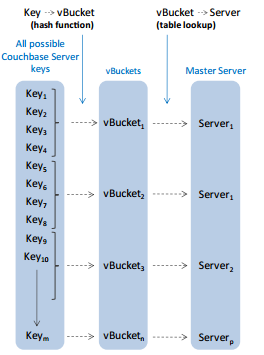
\includegraphics[width=0.4\textwidth]{img/vbucket2}
	\caption{ Couchbase Key, Bucket and   vBucket ~\cite{couchbasedocs}}
	\label{fig:cb-vbucket}
\end{figure}

%where is reference of images



\subsubsection{Querying and Indexing}

 In Couchbase, views are used to create indexes and query the data. Depending on the format and structure of the data, an index is created by the view. when the expiration pager operates to remove a document from the database, then the documents are removed from indexes. Views are used for various purposes such as indexing, querying, producing lists producing tables, filtering and extracting information from the database etc. Multiple views create multiple indexes for storing the data. Views are defined in a special kind of document called \textit{design document}~\ref{fig:cb-views-design}. These documents are bounded to a single bucket and cannot be executed from other buckets. 
 
\paragraph{Mapreduce:} 
The mapreduce reads the entire dataset, in parallel across the cluster. Similarly, in Couchbase views, all the documents are processed with respect to each view. The design document holds JavaScript code that implements mapreduce operations. Couchbase uses incremental mapreduce where the index is incrementally updated as the bucket changes. The Mapreduce is achieved by two functions \textit{map} and \textit{reduce}. 
\begin{itemize}
\item {The map function:}
The map function takes the document and its metadata as the required parameters for initial processing. It provides structure and format of output of a view. The output is depends on the filter used in \textit{emit()} function inside  the map function. Each \textit{emit()} function returns a single row but can be called multiple times inside a single map function. The output of emit function is sent to reduce function if reduce is defined otherwise the output will be key/value pair. 

\item {The reduce function:}
The \textit{reduce} function is used to aggregate the numeric value generated in map phase. Couchbase has built-in reduce functions like \textit{\_count}, \textit{\_sum} and \textit{\_stats} aggregation.

\end{itemize}
Table ~\ref{tbl:cb-mapreduce} illustrates an example of MapReduce  in Couchbase. At the map phase, all the \textit{id}'s of documents that contains \textit{doctype} value "closed\_auctions" and \textit{price} value greater than 40 is emmited. In \textit{reduce}, total number of ids are counted.

%end here from benchmarking sections.
\begin{table}[h]
\begin{longtable}{c|c}
	\caption{Mapreduce in Couchbase}
	\label{tbl:cb-mapreduce}\\
	\textit{map()} & \textit{reduce()}\\
	\hline
\begin{minipage}{.6\textwidth}
\begin{fakeJSON}[label=cb-mapreduce-map,basicstyle =\scriptsize]
function (doc, meta) {
   if(doc.doctype && doc.doctype=="closed_auctions"){
     if(doc.price){
       if(doc.price > 40) {
	      emit(meta.id,null)
     	}
    }
  }
}

\end{fakeJSON}	
\end{minipage} &
\begin{minipage}{.2\textwidth}
\begin{fakeJSON}[label=cb-mapreduce-reduce]
	_count
\end{fakeJSON}
\end{minipage}\\
\end{longtable}
\end{table}

\par
%start here 
\paragraph{Query:}
 In contrast to MongoDB,  Couchbase's queries are closely associated with client SDK where each operations has to perform through SDKs. On-demand query language  named "N1QL" is also in  progress of development but still stable version has to be released~\cite{couchbasen1ql}.
\par
 Query in Couchbase is done against pre-materialize views through REST API or SDK. Different query options like \textit{limit}, \textit{group\_level}, \textit{key}, \textit{keys}, \textit{skip}, etc can be used in view to get required result. 
 
   
 
 
 
 
 
 
 
 
 
 
 
 
 
 
 
 
 
 
 
 
 
 
 

	